\documentclass[12pt, notitlepage, final]{article} 

\newcommand{\name}{Vince Coghlan}

%\usepackage[dvips]{graphics,color}
\usepackage{amsfonts}
\usepackage{amssymb}
\usepackage{amsmath}
\usepackage{latexsym}
\usepackage{enumerate}
\usepackage{amsthm}
\usepackage{nccmath}
\usepackage{setspace}
\usepackage[pdftex]{graphicx}
\usepackage{epstopdf}
\usepackage[siunitx]{circuitikz}
\usepackage{tikz}
\usepackage{float}
\usepackage{cancel} 
\usepackage{setspace}
\usepackage{overpic}
\usepackage{mathtools}
\usepackage{listings}
\usepackage{color}
\usepackage{qtree}
%\usepackage{gensymb}

\usetikzlibrary{calc}
\usetikzlibrary{matrix}
\usetikzlibrary{positioning}

\numberwithin{equation}{section}
\DeclareRobustCommand{\beginProtected}[1]{\begin{#1}}
\DeclareRobustCommand{\endProtected}[1]{\end{#1}}
\newcommand{\dbr}[1]{d_{\mbox{#1BR}}}
\newtheorem{lemma}{Lemma}
\newtheorem*{corollary}{Corollary}
\newtheorem{theorem}{Theorem}
\newtheorem{proposition}{Proposition}
\theoremstyle{definition}
\newtheorem{define}{Definition}
\newcommand{\column}[2]{
\left( \begin{array}{ccc}
#1 \\
#2
\end{array} \right)}

\newdimen\digitwidth
\settowidth\digitwidth{0}
\def~{\hspace{\digitwidth}}

\setlength{\parskip}{1pc}
\setlength{\parindent}{0pt}
\setlength{\topmargin}{-3pc}
\setlength{\textheight}{9.0in}
\setlength{\oddsidemargin}{0pc}
\setlength{\evensidemargin}{0pc}
\setlength{\textwidth}{6.5in}
\newcommand{\answer}[1]{\newpage\noindent\framebox{\vbox{{\bf ECEN 5018 Spring 2014} 
\hfill {\bf \name} \vspace{-1cm}
\begin{center}{Homework \#6}\end{center} } }\bigskip }

\DeclareMathOperator*{\argmin}{arg\,min}

%absolute value code
\DeclarePairedDelimiter\abs{\lvert}{\rvert}%
\DeclarePairedDelimiter\norm{\lVert}{\rVert}
\makeatletter
\let\oldabs\abs
\def\abs{\@ifstar{\oldabs}{\oldabs*}}
%
\let\oldnorm\norm
\def\norm{\@ifstar{\oldnorm}{\oldnorm*}}
\makeatother

\def\dbar{{\mathchar'26\mkern-12mu d}}
\def \Frac{\displaystyle\frac}
\def \Sum{\displaystyle\sum}
\def \Int{\displaystyle\int}
\def \Prod{\displaystyle\prod}
%\def \P[x]{\Frac{\partial}{\partial x}}
%\def \D[x]{\Frac{d}{dx}}
\newcommand{\PD}[2]{\frac{\partial#1}{\partial#2}}
\newcommand{\PF}[1]{\frac{\partial}{\partial#1}}
\newcommand{\DD}[2]{\frac{d#1}{d#2}}
\newcommand{\DF}[1]{\frac{d}{d#1}}
\newcommand{\fix}[2]{\left(#1\right)_#2}
\newcommand{\ket}[1]{|#1\rangle}
\newcommand{\bra}[1]{\langle#1|}
\newcommand{\braket}[2]{\langle #1 | #2 \rangle}
\newcommand{\bopk}[3]{\langle #1 | #2 | #3 \rangle}
\newcommand{\Choose}[2]{\displaystyle {#1 \choose #2}}
\newcommand{\proj}[1]{\ket{#1}\bra{#1}}
\def\del{\vec{\nabla}}
\newcommand{\avg}[1]{\langle#1\rangle}
\newcommand{\piecewise}[4]{\left\{\beginProtected{array}{rl}#1&:#2\\#3&:#4\endProtected{array}\right.}
\newcommand{\systeme}[2]{\left\{\beginProtected{array}{rl}#1\\#2\endProtected{array}\right.}
\def \KE{K\!E}
\def\Godel{G$\ddot{\mbox{o}}$del}

%\onehalfspacing

\begin{document}

\answer{}

\textbf{1.} Consider an anonymous routing/congestion game that is parameterized as follows:
\begin{itemize}
  \item{A finite set of resources $\mathcal{R}$.}
  \item{A congestion function for each resource $r$ of the form $c_r : \{0,1,2,...\} \rightarrow R$.
    The cost $c_r(k)$ is the congestion on resource/road $r$ when there are $k$ users.  In this
    formulation, congestion on a particular resource/road only depends on the number of users on
    that road not which specific users, i.e., users are anonymous.}
  \item{A finite set of players $N = \{1,2,...,n\}$.}
  \item{A finite action set of each player $\mathcal{A}_i \subseteq 2^\mathcal{R} :$ An action
    $a_i \in \mathcal{A}_i$ is just a collection of resources, i.e., $a_i \subseteq \mathcal{R}$.
    Let $\mathcal{A} := \mathcal{A}_1 \times ... \times \mathcal{A}_n$ represent the set of joint
    actions.}
  \item{A cost function for each player $i$ of the form $J_i : \mathcal{A} \rightarrow R$ that each
    player seeks to minimize.  The specific form of the cost function is
    \[
      J_i(a_i,a_{-i}) = \sum_{r \in a_i}c_r(|a|_r)
    \]
    where $|a|_r$ represents the number of players that choose resource $r$ in the action profile $a$,
    i.e.,
    \[
      |a|_r=|\{j\in N:r\in a_j\}|
    \]
  }
\end{itemize}
\begin{enumerate}[(a)]
  \item{Consider the following two player congestion game:}
  \begin{itemize}
    \item{$\mathcal{R} = \{r_1,r_2\}$.}
    \item{$N=\{1,2\}$.}
    \item{$\mathcal{A}_i \subseteq 2^\mathcal{R}$: (a player can select either resource $r_1$ or
      $r_2$ but not both)}
  \end{itemize}
  Write down the payoff matrix for this two player routing game.  Prove that a pure Nash equilibrium must
  exist irrespective of the congestion functions for route $r_1$ and $r_2$.

  \begin{center}
  \begin{tabular}{r |c|c|}
    \multicolumn{1}{r}{}
    & \multicolumn{1}{c}{$r_1$}
    & \multicolumn{1}{c}{$r_2$}\\
    \cline{2-3}
    $r_1$ & $c_{r_1}(2), c_{r_1}(2)$ & $c_{r_1}(1), c_{r_2}(1)$\\
    \cline{2-3}
    $r_2$ & $c_{r_2}(1), c_{r_1}(1)$ & $c_{r_2}(2), c_{r_2}(2)$\\
    \cline{2-3}
  \end{tabular}
  \end{center}

  Note that this follows the form:
  \begin{center}
  \begin{tabular}{r |c|c|}
    \multicolumn{1}{r}{}
    & \multicolumn{1}{c}{$r_1$}
    & \multicolumn{1}{c}{$r_2$}\\
    \cline{2-3}
    $r_1$ & a, a & b, c\\
    \cline{2-3}
    $r_2$ & c, b & d, d\\
    \cline{2-3}
  \end{tabular}
  \end{center}

  Which we can prove is a potential game with a $\Phi$:

  \begin{center}
  \begin{tabular}{r |c|c|}
    \multicolumn{1}{r}{}
    & \multicolumn{1}{c}{$r_1$}
    & \multicolumn{1}{c}{$r_2$}\\
    \cline{2-3}
    $r_1$ & a-c & 0\\
    \cline{2-3}
    $r_2$ & 0& d-b\\
    \cline{2-3}
  \end{tabular}
  \end{center}

  Since this is a potential game, we can begin from an arbitrary $a$ and each step
  will reduce a player's cost.  We know that $\Phi$ is going to be finite and eventually
  will be minimized, at which point no player will have any incentive to deviate, a NE.

  \item{Consider any arbitrary routing game with $n$ players:}
    \begin{itemize}
      \item{$\mathcal{R}=\{r_1,...,r_m\}$}.
      \item{$N=\{1,...,n\}$}.
      \item{$\mathcal{A} \subseteq 2^\mathcal{R}$}.
    \end{itemize}
    Consider the following two potential functions:
    \[
      \Phi^1(a)=\sum_{r\in \mathcal{R}}|a|_r \cdot c_r (|a|_r)
    \]
    \[
      \Phi^2(a)=\sum_{r\in \mathcal{R}}\sum_{k=1}^{|a|_r}c_r(k)
    \]
    Let $a$ and $a'=(a_i',a_{-i})$ be any two routing profiles that differ by a unilateral deviation.
    Prove or disprove the following statement:
    \[
      U_i(a) - U_i(a')=\Phi^1(a)-\Phi^1(a')
    \]

    We can see that:
    \[
      U_i(a) - U_i(a')=c_r(|a|_r)-c_{r'}(|a|_{r'}+1)
    \]
    \[
      c_r(|a|_r)-c_{r'}(|a|_{r'}+1) = \sum_{r\in\mathcal{R}}|a|_r\cdot c_r(|a|_r) - \sum_{r\in\mathcal{R}}|a|_{r'}\cdot c_{r'}(|a|_{r'})
    \]
    Only two of the resources will not cancel out when we add these together:
    \[
      c_r(|a|_r)-c_{r'}(|a|_{r'}+1) = |a|_r\cdot c_r(|a|_r)+|a|_{r'}\cdot c_{r'}(|a|_{r'})-|a|_{r}\cdot c_{r}(|a|_{r}-1)-|a|_{r'}\cdot c_{r'}(|a|_{r'}+1)
    \]
    These are not the same, which exemplifies that the system cost may not be optimized when players optimise
    their own personal utilities.

  \item{Prove or disprove the following statement:}
    \[
      U_i(a)-U_i(a')=\Phi^2(a)-\Phi^2(a')
    \]

    A similar method as above:
    \[
      c_r(|a|_r)-c_{r'}(|a|_{r'}+1)=\sum_{r\in \mathcal{R}}\sum_{k=1}^{|a|_r}c_r(k)-\sum_{r\in \mathcal{R}}\sum_{k=1}^{|a|_{r'}}c_{r'}(k)
    \]
    Once again every term is the same exept for the new resource $r'$, which leaves us with:
    \[
      c_r(|a|_r)-c_{r'}(|a|_{r'}+1)=c_r(|a|_r)-c_{r'}(|a|_{r'}+1)
    \]
    Hence these are equal.

  \item{Prove that a pure Nash equilibrium must exist in \textit{any} congestion game.}
    Our previous proof tells us that every congestion game is a potential game.  Meaning that any move
    by a player that optimises his utility will also optimise the potential.  Since potential is a finite
    function, this must end at some point, a point where no move will increase the potential, meaning no move
    increase any agent's utility, meaning no agent has an incentive to deviate, a NE.

  \item{Derive an anonymous tolling scheme, i.e., $t_r:\{0,1,2,...\}\rightarrow R$ for each resource $r\in R$
    such that the resulting game where player's cost functions are now}
    \[
      \tilde{J}(a_i,a_{-i})=\sum_{r\in a_i}(c_r(|a|_r+t_r(|a|_r)))
    \]
    We now have:
    \[
      U_i(a')-U_i(a)=c_r(|a|_r)+t_r(|a|_r)-c_{r'}(|a|_{r'}+1)-t_{r'}(|a|_{r'}+1)
    \]
    Now we can set the potential game requirement:
    \[
      c_r(|a|_r)+t_r(|a|_r)-c_{r'}(|a|_{r'}+1)-t_{r'}(|a|_{r'}+1)=
    \]
    \[
      |a|_r\cdot c_r(|a|_r)+|a|_{r'}\cdot c_{r'}(|a|_{r'})-|a|_{r}\cdot c_{r}(|a|_{r}-1)-|a|_{r'}\cdot c_{r'}(|a|_{r'}+1)
    \]
    Any $t_r$ that satisfies this requirement will be a potential game.  For example, you could set one of these
    tabularxes to 0, and the other to the rest of this expression.
\end{enumerate}

\textbf{2.} The setup for distributed routing is as follows:
\begin{itemize}
  \item{There are 3 parallel roads and 60 vehicles.}
  \item{Let $n_r$ be the number of vehicles on road $r$.  The congestion on each road is:}
    \[
      c_1(n_1)=40+n_1
    \]
    \[
      c_2(n_2)=20+n_2^2
    \]
    \[
      c_3(n_3)=1+5n_3^2
    \]
    Write a Matlab script to solve distributed routing using JSFP with Inertua ($\epsilon=1$).
  \item{Display both final congestion and number of vehicles on each road.}
  \item{For one particular player, display the regret for each action as a function of the interation
    number (all on same plot)}
  \item{Confirm that the congestion on each road is (approximately) equal}.
\end{itemize}

\begin{figure}[H]
\begin{center}
\caption{Congestion}
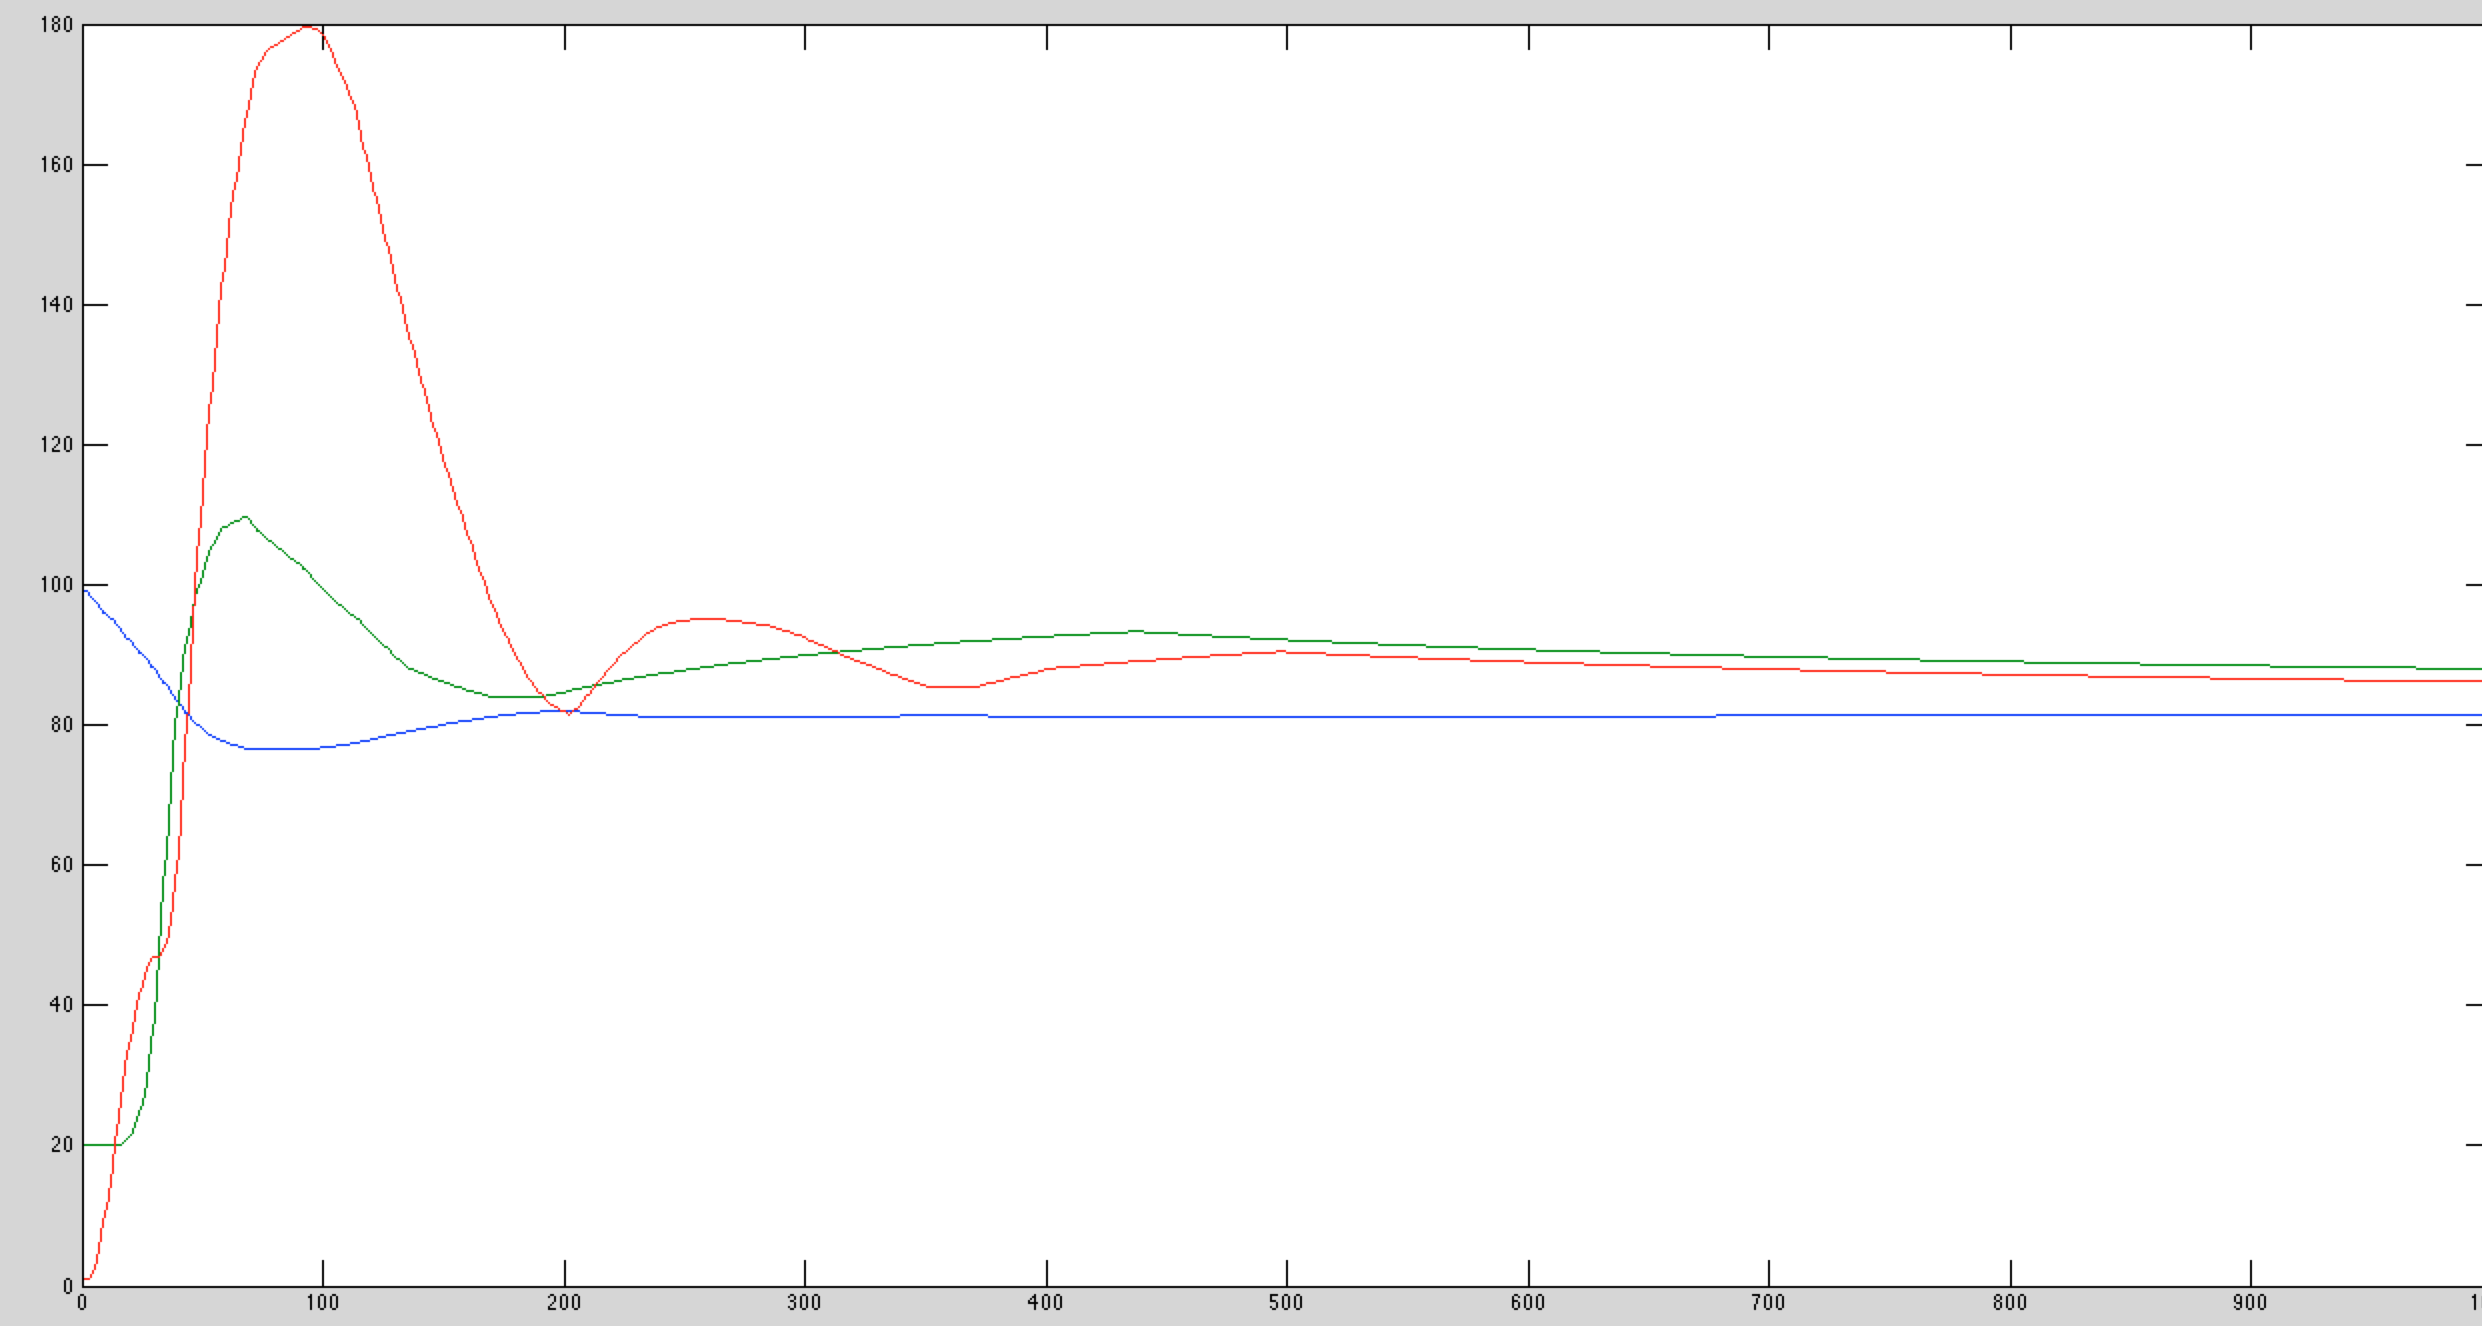
\includegraphics[width=14cm]{f1}
\end{center}
\end{figure}
\begin{figure}[H]
\begin{center}
\caption{Number of Vehicles on each road}
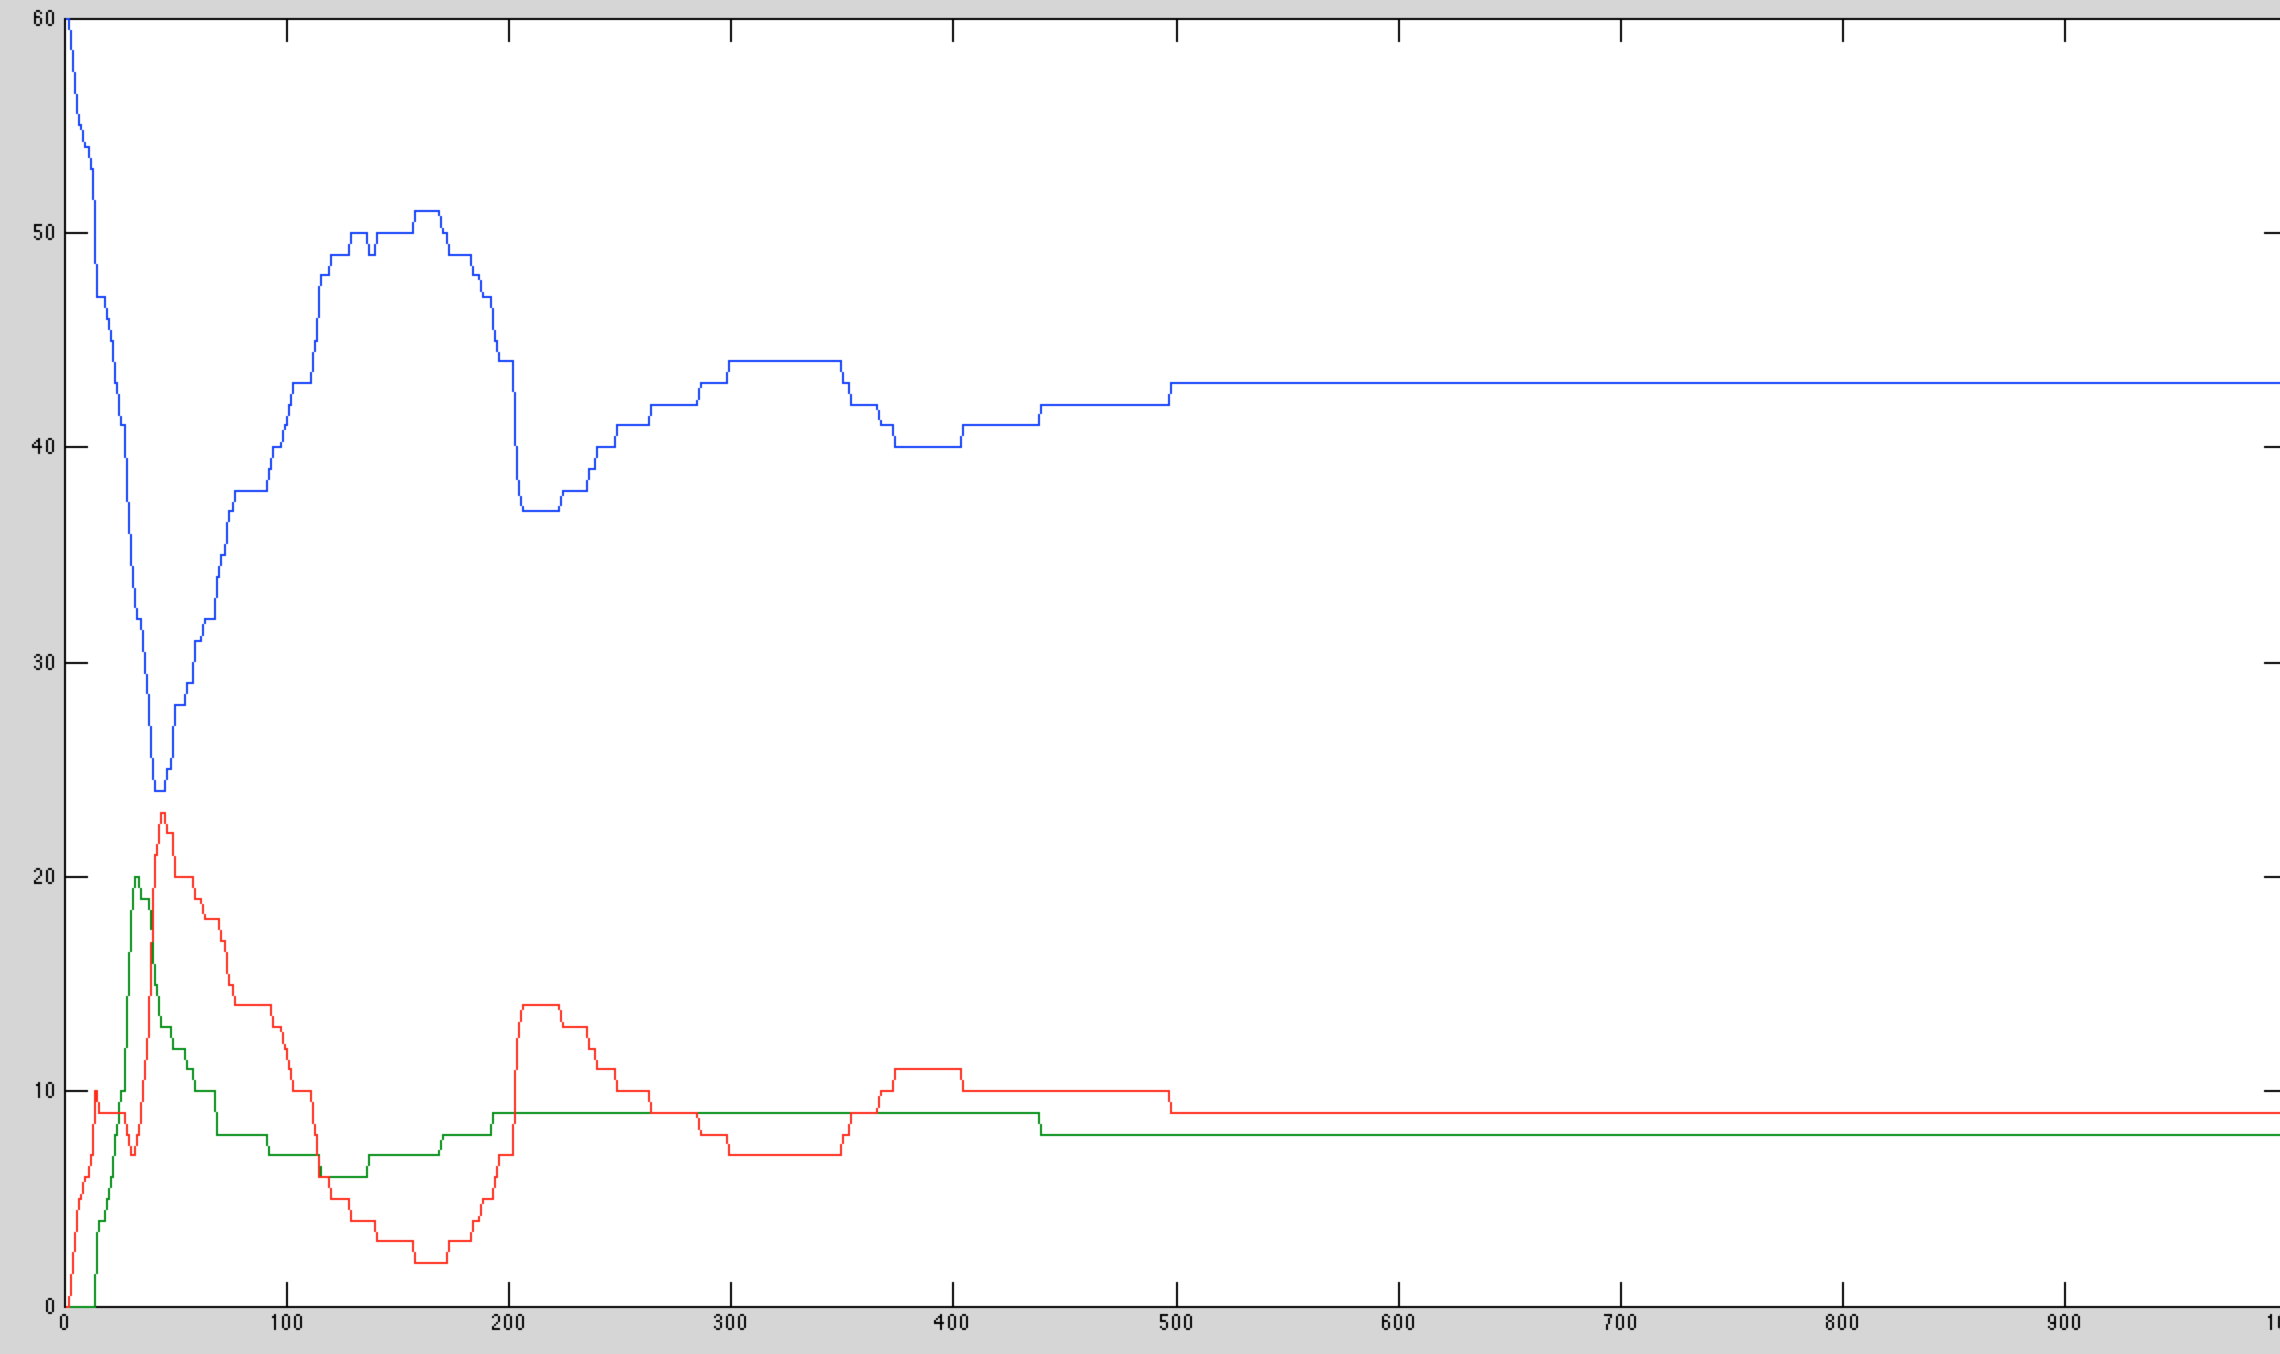
\includegraphics[width=14cm]{f2}
\end{center}
\end{figure}
\begin{figure}[H]
\begin{center}
\caption{Regret}
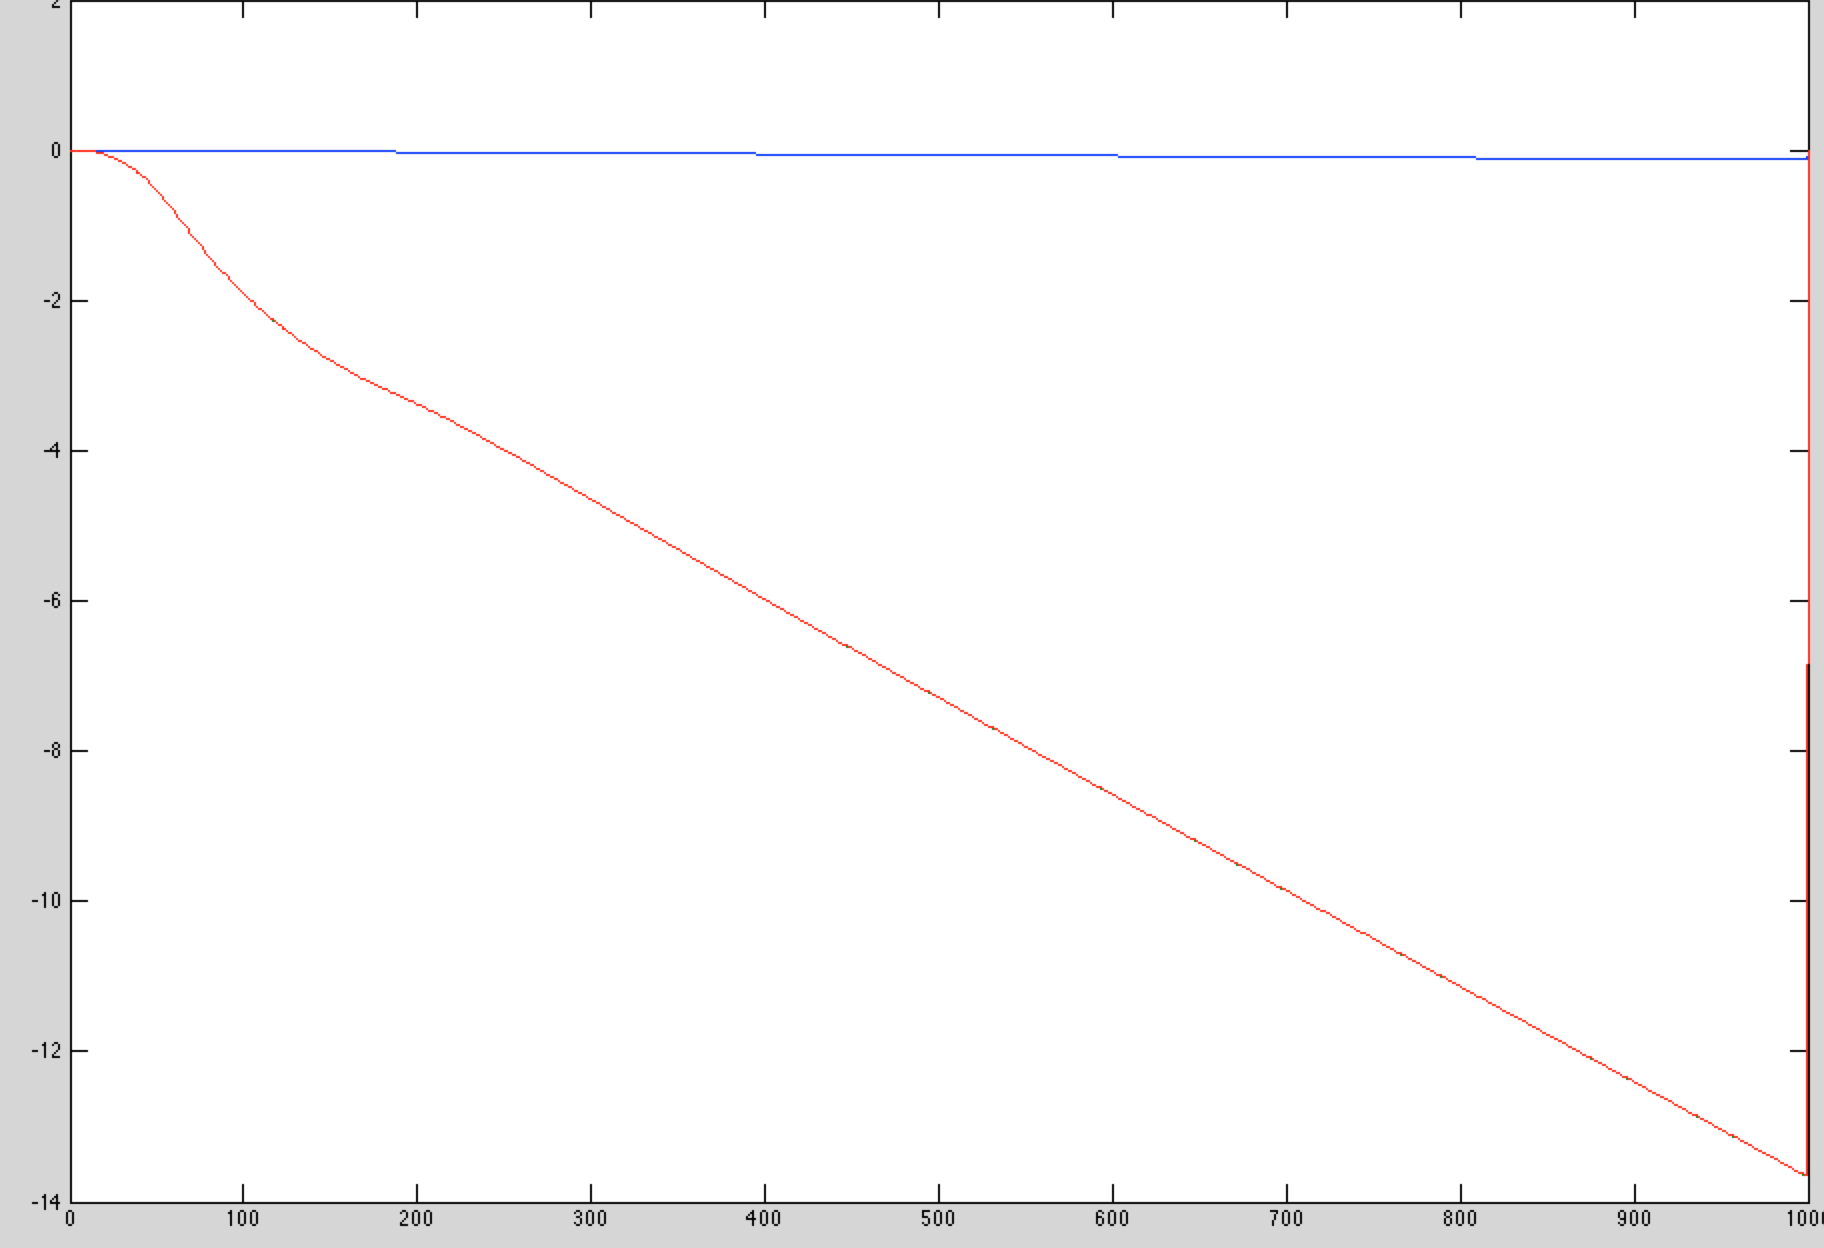
\includegraphics[width=14cm]{f3}
\end{center}
\end{figure}
The reason one of the resources' regrets barely drops at all is since every agent began on the same
resource, the cost was initially very very high, and regret wont drop for a while.

The congestion on each road is around 82-86, which is indeed approximately equal.

\textbf{3.} The table below shows a global performance measure as a function of the joint actions of
two players.  The action '$\emptyset$' refects the \textit{absense} of that player.

  \begin{center}
  \begin{tabular}{r |c|c|c|}
    \multicolumn{1}{r}{}
    & \multicolumn{1}{c}{$\emptyset$}
    & \multicolumn{1}{c}{L}
    & \multicolumn{1}{c}{R}\\
    \cline{2-4}
    $\emptyset$ & 0 & 1 & 2\\
    \cline{2-4}
    $T$ & 7 & 8 & 3\\
    \cline{2-4}
    $B$ & 6 & 5 & 7\\
    \cline{2-4}
  \end{tabular}\\
  \vspace{2mm}
  \hspace{6mm}$W(a_{ROW},a_{COL})$
  \end{center}

  \begin{enumerate}[(a)]
    \item{Fill in the matrix table below using the \textbf{marginal contribution utility} to derive \textbf{both}
      utility functions $u_{ROW}(\cdot)$ and $u_{COL}(\cdot)$.}

  Each player will pay his marginal contribution:

  \begin{center}
  \begin{tabular}{r |c|c|}
    \multicolumn{1}{r}{}
    & \multicolumn{1}{c}{L}
    & \multicolumn{1}{c}{R}\\
    \cline{2-3}
    T & 7,1 & 1,-4\\
    \cline{2-3}
    B & 4,-1 & 5, 1\\
    \cline{2-3}
  \end{tabular}
  \end{center}
  \item{The efficient joint action (T,L) should be a Nash equilibrium of the resultimg game.  Is it the \textit{only}
    Nash equilibrium?}\\
  There is another NE, (B, R).  A high payoff, but not the optimal.

  \item{Fill in the matrix table below using the \textit{Shapley value utility} to derive \textit{both} utility
  functions $u_{ROW}(\cdot)$ and $u_{COL}(\cdot)$.}

  The Shapley value utility will assign the average margian utility in getting to an action.  For example, when
  (T,L) is played, the payoff is 8, and player 1's average marginal utility to get there is:
  \[
    \frac{1}{2}((8-5) + (8-1))=5
  \]
  The entire thing can be filled in:
  \begin{center}
  \begin{tabular}{r |c|c|}
    \multicolumn{1}{r}{}
    & \multicolumn{1}{c}{L}
    & \multicolumn{1}{c}{R}\\
    \cline{2-3}
    T & 5,3 & -3/2,-9/2\\
    \cline{2-3}
    B & -3/2,1/2 & 3/2, 9/2\\
    \cline{2-3}
  \end{tabular}
  \end{center}


  \end{enumerate}

\textbf{4.} Consider any $4 \times 4$ Sudoku puzzle as illustrated below

\[
  \begin{pmatrix}
    0&1&0&0\\
    0&2&0&0\\
    2&0&0&0\\
    0&0&3&0
  \end{pmatrix}
\]

Where a 0 indicates that the box is initally empty. Model the Sudoku puzzle as a game with the
following specifications:
\begin{itemize}
  \item{Boxes with a 0 are modeled as players in a game, i.e., there are 12 players in the above game}
  \item{Actions of each player $i\in N$ is $\mathcal{A}_i=\{1,2,3,4\}$}
  \item{Cost functions of each player $i\in N$ is}
    \[
      J_i(a_i,a_{-i}) = (\#\text{ repetitions in a row})+(\#\text{ repititions in col})+(\#\text{ repetitions in } 2\times2 \text{ box})
    \]
\end{itemize}

\begin{enumerate}
  \item{Does a Nash equilibrium always exist, i.e., for any initial configuration?}\\
    I think it does, because this is a potential game.  If we set the potential function to the sum of
    these utilities for every player, we can see that if a player increases his own utility, then all
    other player's utilities will also increase, i.e., if a player makes a decision that is good for him,
    all other players in his set will also benifit.  If this is indeed a potential game, then a NE would
    have to exist for this finite potential function.

   \item{Is a solution to the Sudoku puzzle a Nash equilibrium?}\\
     Yes, since if we are at a solution, everyone's cost is 0.  if one player were to deviate they would
     create a repition in all 3 categories and their new cost would be 3.

   \item{Is a Nash equilibrium a solution to the Sudoku puzzle?}\\
     Not necessarily, It is quite trivial to create a Sudoku puzzle that is impossible to solve, and thus
     its NE would not be a solution.
 \end{enumerate}

\textbf{5.} Write a Matlab script to solve $4 \times 4$ Sudoku using Cournot best reply inertia.  Please structure
your script according to the following specifications:
\begin{itemize}
  \item{Use the game specifications highlighted above}
  \item{Have as an input the $4 \times 4$ matrix starter that specifies fixed cell values.  For example}
  \[
    \text{starter}=\begin{pmatrix}
    0&1&0&0\\
    0&2&0&0\\
    2&0&0&0\\
    0&0&3&0
  \end{pmatrix}
  \]
  fixes the values of specific cells.  A "zero" indicates that cell is free to change values, i.e., it is
  a free agent.
  \item{Have as an input the inertia probability $p$ (i.e., probability of repeating the previous actions}.
  \item{When completed, display the solved puzzle and number of iterations}.
\end{itemize}

solutions are:
  \[
    \begin{pmatrix}
    3&1&2&4\\
    4&2&1&3\\
    2&3&4&1\\
    1&4&3&2
  \end{pmatrix}
  \]
  \[
    \begin{pmatrix}
    4&1&2&3\\
    3&2&1&4\\
    2&3&4&1\\
    1&4&3&2
  \end{pmatrix}
  \]

  Finishes in 60-70 iterations

\end{document}
